\documentclass[
paper=a4,
draft=false,%     Entwurfsmodus
fontsize=10pt% Größe der Grundschrift
]{scrartcl}

\def\logo{logos/colorlogo_rgb}% Logo bei Normaldruck.
%\def\logo{logos/colorlogo_cmyk}% Logo bei Profidruck.

\usepackage{cca-page} % design nach vorschrift

\begin{document}

\title{%
An die:\\
Contao Association\\
Sonnhalderain 15\\
CH - 3250 Lyss\\
\href{http://c-c-a.org}{\includegraphics[width=.6\textwidth]{\logo}}\\
Antrag auf Förderung des Contao Composer Projekts durch die Contao Association\\%
}
\date{24 Oktober 2014}
\author{Contao-Community-Alliance}
\maketitle

\pagebreak

% --------------------------------------------------------------------------------
%
%     Historie
%
% --------------------------------------------------------------------------------

\section*{Historie}
\label{sec:history}

\begin{tabular*}{\textwidth}{@{\extracolsep{\fill} }llp{.7\textwidth}}
\textbf{Version} & \textbf{Datum} & \textbf{Zusammenfassung} \\
\hline
1   & 24. Oktober 2014 & Erste Version, eingereicht am 24. Oktober 2014 an die Contao Association. \\
\hline
1.1 & -                & Korrektur diverser Rechtschreibfehler. \newline
                         Hinzufügen von Yanick \uquot{Toflar} Witschi als Unterstützer. \newline
                         Weitere Fußnoten eingefügt. \\
\end{tabular*}

\pagebreak

% --------------------------------------------------------------------------------
%
%     Präambel
%
% --------------------------------------------------------------------------------

\section*{Präambel}
\label{sec:preamble}

Gefördert werden soll das Contao Composer Projekt, das durch die CCA betreut wird. \\
Das Projekt besteht aus mehreren Teilprojekten:

\begin{itemize}
\item ...dem Contao Composer Client (nachfolgend CCC benannt), \\
dieser stellt die Integration von Composer in das Contao Backend zur Verfügung. \\
Den meisten Nutzern dürfte der CCC als Menüpunkt \uquot{Paketverwaltung} bekannt sein.
\item ...dem Contao Composer Plugin (nachfolgend CCP benannt), \\
dieser stellt in Composer die Funktion zur Verfügung, Contao Erweiterungen über Composer zu installieren.
\item ...dem Contao Composer Repository (nachfolgend CCR benannt), \\
dies ist ein an das Contao Ökosystem angepasster Paketserver auf Basis von Packagist.
\item ...dem Composer.json Generator (nachfolgend CJG benannt), \\
hierbei handelt es sich um ein Web-Tool, dass den Entwicklern den Umstieg zu Composer erleichtern soll.
\item ...der Contao Composer Dokumentation (nachfolgend CCD benannt).
\end{itemize}

Außerdem umfasst der Antrag folgende weitere Projekte, die unmittelbar mit dem Contao Composer Projekt zusammen hängen oder sogar als \uquot{Nebenprodukt} entstanden sind oder entstehen sollen.

\begin{itemize}
\item Database Update Tool (nachfolgend DUT benannt), \\
ein eigenständiges Tool um das Datenbankupdate durchzuführen. In Contao ist das Datenbankupdate an das Install-Tool oder die Paketverwaltung gebunden. Das DUT soll das Datenbankupdate als eigenständige Komponente anbieten. Sowohl im Backend, als auch im CCC, so wie auf der Konsole!
\item Migration Toolkit (nachfolgend MTK benannt), ist ein Tool, inspiriert von Doctrine Migrations\footnote{\hreflink{http://www.doctrine-project.org/projects/migrations.html}}, allerdings ist es allgemeiner gehalten und soll als Ersatz für die unspezifizierte \texttt{runone.php} dienen um in Zukunft fehlerhafte oder inkomplette Datenupgrades zu verhindern (bislang hat nur der Core eine \uquot{richtige} Datenmigration vornehmen können).
\end{itemize}

\subsection*{Welches Ziel hat dieser Antrag?}

Bereits Anfang 2014\footnote{\hreflink{https://contao.org/de/news/zwischenmeldung-zum-extension-repository-3.html}} haben wir in einem klärenden Gespräch festgestellt, dass der CCC zwar schon funktioniert, aber es vor allem am Ökosystem hapert. Das vorhandene Ökosystem rund um das ER2 ist deutlich umfangreicher als das, was wir um den CCC bisher aufbauen konnten.

Dieser Antrag befasst sich - soweit es aktuell planbar ist - damit, das Ökosystem rund um den CCC aufzubauen, so dass wir in absehbarer Zeit - 2015/2016 - das alte ER2 auch tatsächlich ablösen können.

Vor allem die \uquot{mangelnde} Usability, die in den Kommentaren des Newsbeitrags vom 20. März 2014 so oft angesprochen wurde möchten wir \uquot{aus dem Weg schaffen}.

\pagebreak
\tableofcontents
\pagebreak

% --------------------------------------------------------------------------------
%
%     tl;dr - Zusammenfassung
%
% --------------------------------------------------------------------------------

\section[tl;dr - Zusammenfassung]{tl;dr - Zusammenfassung\footnote{Too long; didn't read -
\hreflink{http://en.wikipedia.org/wiki/Wikipedia:Too\_long;\_didn't\_read}}}
\label{sec:summary}

\textit{Der Antrag ist dir zu lang? Hier findest du eine Zusammenfassung!}

Wie im Präambel beschrieben umfasst der Antrag das gesamte Contao Composer Projekt. Nicht nur aktuelle, auch kurzfristige, sowie mittelfristige und langfristige Ziele.

Der Antrag verfolgt dabei 2 Ziele:
Erstens wollen wir die Kritiken aufgreifen und die Bedienbarkeit verbessern. Dies soll zum einen durch Verbesserung der Oberfläche, zum anderen durch bereitstellen einer Dokumentation geschehen.
Zweitens wollen wir das Ökosystem aufbauen, dass das aktuelle ER2 zur Zeit bietet, so dass wir im Zeitrahmen 2015/2016 ernsthaft darüber reden können, das alte ER2 abzulösen. An dieser Stelle erst mal Entwarnung: Das ER2 wird uns noch einige Jahre erhalten bleiben um älteren Contao Installationen nicht \uquot{den Stecker zu ziehen}.

Composer ist nicht ganz unumstritten, da es teilweise sehr ressourcenhungrig ist. Allerdings stehen uns kaum Alternativen zur Verfügung. Native Paketverwaltungen wie PEAR/PECL fallen auf Shared Hostings weg. Da Composer rein in PHP geschrieben ist, lässt es sich auf nahezu allen PHP Plattformen betreiben. Man muss auch sagen dass sich Composer in den vergangenen 2 Jahren sehr gut weiterentwickelt hat und deutlich verbessert wurde. Die Systemanforderungen sind gesunken und die Performance gestiegen. Wir setzen hier auf die Erfahrung und Arbeit von etwa 10 Entwicklern die regelmäßig zu Composer beitragen. Und über 100 weiteren Entwicklern die hier und da was zum Composer beitragen\footnote{\hreflink{https://github.com/composer/composer/graphs/contributors}}.

Wir sind nicht die einzigen die auf den \uquot{Composer Zug} aufspringen. Drupal, Typo3 NEOS, Laravel, Yii, Doctrine, Symfony und zahllose weitere Projekte nutzen Composer. Es gibt bereits über 40.000 Pakete auf packagist.org zu finden! Es ist anzunehmen, dass durch die große Verbreitung auch die Shared Hoster zukünftig dazu gezwungen sein werden, Composer besser zu unterstützen.

Der Umfang des Antrags würde das Jahresbudget der Association deutlich sprengen. Deshalb wird dieser Antrag in \uquot{Entwicklungspakete} aufgesplittet, die dann zur Förderung eingereicht werden oder durch andere Unternehmen gefördert werden können.
Für die Community ist die Gesamtheit des Antrags aber immer noch ein Leitfaden, was alles noch folgen wird.
Dabei sollte jedoch beachtet werden, dass der Antrag nicht starr ist. Einige mittel- und langfristige Positionen sind noch nicht vollständig ausgearbeitet und geplant und das ist auch beabsichtigt. Die weiterführenden Positionen wollen wir in Zusammenarbeit mit der Community ausarbeiten und planen.

Dabei helfen uns die \uquot{Entwicklungspakete} die zeitgleich zu einem agilen Entwicklungsmodel führen. Nach jedem Entwicklungsschritt können wir ein Resümee ziehen und gemeinsam die nächsten Schritte planen.

\newpage

% --------------------------------------------------------------------------------
%
%     Composer, was ist das?
%
% --------------------------------------------------------------------------------

\section{Composer, was ist das?}
\label{sec:why-composer}

\subsection{Verwirrende Nomenklatur - Was ist Composer?}

\uquot{Composer} hört man als Begriff in der Contao Community in letzter Zeit sehr häufig. Dabei stammt Composer gar nicht aus dem Contao Umfeld. Composer\footnote{\hreflink{https://getcomposer.org}} ist eine sogenannte Paketverwaltung speziell für PHP - nicht nur speziell für Contao. Das Composer Projekt wurde Anfang 2011 von Nils Adermann und Jordi Boggiano initiiert und erfreut sich seit 2012 wachsender Beliebtheit und Verbreitung. Abgesehen von PEAR\footnote{\hreflink{http://pear.php.net/}}, welches nativ auf dem System ausgeführt wird, gab es für PHP über die letzten Jahre hinweg keine vernünftige Paketverwaltung. Composer ist vollständig in PHP geschrieben und lässt sich daher im Gegensatz zu PEAR auch auf restriktiven Systemen (Shared Hoster) verwenden. Zum Composer-Ökosystem gehört unter anderem Packagist\footnote{\hreflink{https://packagist.org/}}, das als primäres Repository für Pakete dient.

\begin{info}
In diesem Dokument ist mit \textbf{Composer} immer das Composer Projekt von Nils und Jordi gemeint.
In der Contao Community ist damit umgangssprachlich der \textbf{Contao Composer Client} gemeint.
Leider führt das des öfteren immer wieder zu Verwirrung. \\
\\
Unter dem Begriff \textbf{Contao Composer Projekt} - umgangssprachlich auch als \textbf{Composer Projekt} abgekürzt - vereinen wir alle zugehörigen Teilprojekte (siehe \nameref{sec:preamble}).
\end{info}

\subsection{Was ist aus dem ER3 geworden?}

Das ER3, auch bekannt als RFCCC-1\footnote{\hreflink{https://c-c-a.org/rfccc1}} war ein Vorstoß aus 2011 um den Weg für einen neuen Erweiterungskatalog zu ebnen, im gleichen Jahr hat Composer das Licht der Welt erblickt. Im Jahr 2012 hatte Composer dann seinen großen Aufschwung und wir hatten neugierige Blicke auf dieses aufstrebende Projekt geworfen. Anfang 2013 entstand dann die erste Integration von Composer für Contao.

\begin{emquote}{Christian Schiffler, Tristan Lins}
Als wir den RFCCC-1 (ER3 Dokumentation) schrieben, haben wir festgestellt dass die ganze Thematik \uquot{Paketverwaltung und Abhängigkeitsmanagement} technisch deutlich komplexer ist, als es auf den ersten Blick den Eindruck macht. Nils und Jordi haben hier eine großartige Vorarbeit geleistet, viele Stunden investiert und obendrein eine große Anzahl an Mitstreitern um sich geschart die regelmäßig dazu beitragen, Composer zu verbessern - wir gehören auch dazu. Composer mag durchaus auch seine Schwächen haben - bspw. relativ hohe Systemanforderungen - aber wir könnten es auch nicht besser machen, besonders nicht bei gleicher Funktionalität.
\end{emquote}

Für uns war, ist und bleibt Composer aktuell die beste Grundlage die wir nutzen können. Das ER3 ist also nicht gestorben, viel mehr haben wir mit Composer die Grundlage zur Hand, um das ER3 in erschwinglicher Zeit und akzeptablen finanziellen Aufwand darauf aufzubauen.

Schon heute wird der Contao Composer Client in immer mehr Installationen eingesetzt (>15.000 Downloads\footnote{\hreflink{https://c-c-a.org/composer-counter}}). Einige Erweiterungen die bereits über Composer vertrieben werden, werden im ER2 nur noch sporadisch aktualisiert. Andere Erweiterungen sind gar nicht mehr im ER2 verfügbar. Die bekanntesten Vertreter sind vermutlich Avisota und MetaModels, aber auch einige andere Erweiterungen die nicht aus der Hand der Antragsteller stammen, sind nur noch über Composer verfügbar! Bspw. die Contao Bootstrap Erweiterung\footnote{\hreflink{https://packagist.org/packages/contao-bootstrap/}} von David Molineus.

\newpage

% --------------------------------------------------------------------------------
%
%     Vorteile für Nutzer
%
% --------------------------------------------------------------------------------

\section{Vorteile für Nutzer}
\label{sec:pros-for-users}

\begin{minipage}{.02\linewidth}
  \rotatebox{90}{\textbf{tl;dr - Vorteile auf einen Blick}}
\end{minipage}
\begin{minipage}{.98\linewidth}
  \begin{dinglist}{'64}
  \item Abhängigkeitskonflikte zwischen Erweiterungen werden automatisch aufgelöst und nur kompatible Versionen werden installiert - Stichwort: Versionshopping\footnotemark.
  \item Man erhält schneller Updates und Bugfixes, im Idealfall sofort nach dem ein Bug behoben wurde - Stichwort: Semantische Versionierung\footnotemark.
  \item Im \textit{Standalone Modus} kann man eine defekte Installation auch ohne FTP und händische Korrektur wiederherstellen.
  \item Zukunftssicher dank Open Source und einer breiten Entwicklergemeinschaft - 10 aktive und über 100 weitere Entwickler.
  \end{dinglist}
\end{minipage}

\addtocounter{footnote}{-1}
\footnotetext{Unter Versionshopping verstehen wir die Situation, in der das ER2 dauerhaft eine Erweiterung erst upgraden, danach direkt wieder downgraden will und umgekehrt. Versionshopping entsteht, wenn eine Erweiterung von zwei anderen Erweiterungen als Abhängigkeit bezogen wird und dazu auch noch in 2 unterschiedlichen Versionen. Das ER2 springt dann zwischen den 2 angeforderten Versionen der abhängigen Erweiterung stendig hin und her.\vspace*{3mm}\label{fn:versionshopping}}
\stepcounter{footnote}
\footnotetext{\href{http://semver.org/}{SemVer2 (semver.org)} beschreibt eine Art wie man Versionen einer Software festlegt. Der 3. Level einer Version (also der Z Level: x.y.\textbf{Z}) dient dabei zum versionieren von Bugfixes. Im Idealfall hat jeder Bugfix seine eigene Versionsnummer. D.h. verfolgt ein Entwickler dieses Prinzip und hat er einen Bug behoben, kann er ihn auch gleich in einer neuen Version veröffentlichen. Nutzer müssen nicht mehr auf das nächste \uquot{große Release} warten oder sich mühevoll den Bugfix händisch installieren.\vspace*{3mm}\label{fn:semver}}

\textit{Ein schlanker Core und hochwertige/umfangreiche Erweiterungen}, dafür steht Contao seit 2006. Um die Bereitstellung des Erweiterungskatalogs kümmert sich seit geraumer Zeit das so genannte \uquot{Extension Repository 2} - kurz \uquot{ER2}. Das ER2 stellt aktuell die Erweiterungsliste auf Contao\footnote{\hreflink{https://contao.org/de/extension-list.html}}, so wie den Erweiterungskatalog und die Erweiterungsverwaltung im Contao Backend. Doch das ER2 hat seine Schwächen, so werden Abhängigkeiten nicht richtig aufgelöst - Stichwort: Versionshopping\footref{fn:versionshopping} - oder es lassen sich mit der Contao Version oder mit anderen Erweiterungen inkompatible Erweiterungen installieren.

Unterm Strich muss man sagen, dass die Vorteile von Composer primär die Entwickler betreffen. Doch was für den Entwickler ein Vorteil ist, ist letztlich auch für den Nutzer ein Vorteil. Aber auch die Schwächen des aktuellen CCC für die Nutzer sind uns bewusst und gerade diese wollen wir mit Hilfe dieses Antrags beheben. Dazu zählen unter anderem eine deutliche Verbesserung der Übersichtlichkeit beim Finden, Installieren und Verwalten von Erweiterungen. Zum anderen wollen wir die Kompatibilität zu den zahlreichen Shared Hostern erhöhen.

Aber worum geht es konkret?

Durch die veraltete und unzureichende Implementierung der Abhängigkeitsverwaltung im ER2 ist es aktuell möglich, wenn nicht gar wahrscheinlich, dass sich Nutzer Erweiterungen die zu einander oder zur aktuellen Contao Version inkompatibel sind installieren und somit potentiell die Installation lahm legen - Stichwort: \uquot{gelbe Box}. Diese Probleme werden durch Composer weitestgehend vermieden, so lange die Entwickler selbst keinen Mist bauen. Denn Composer hat eine \uquot{strikte} und zugleich \uquot{offener} Auflösung der Abhängigkeiten. Richtig angewendet sorgt das dafür, dass man als Nutzer immer mit dem neuesten, stabilsten und zu meiner Installation kompatiblen Set an Erweiterungen arbeiten kann.

Sollte es dennoch zu Problemen kommen - den auch Composer kann uns nicht vor allen Problemen schützen - und sollte das Backend dann nicht mehr nutzbar sein, kann man mit Hilfe des \textit{Standalone Modus} die defekte Erweiterung auch wieder entfernen und das Backend \uquot{wiederbeleben}. Den \textit{Standalone Modus} kann man sich ähnlich wie das Install Tool vorstellen, nur halt für die Erweiterungsverwaltung. Mit dem ER2 ist dies aktuell nicht möglich und man muss von Hand via FTP nachhelfen. Gerade für nicht-Entwickler ist hier nicht selten Nachfragen im Forum, IRC, Twitter und Co. erforderlich.

Ein weiterer Punkt ist die Veröffentlichung von neuen Versionen. Für Entwickler ist dies aktuell relativ zeitaufwendig, abgesehen vom \uquot{taggen}\footnote{Damit bezeichnet man das Markieren einer Version zu einem gewissen Stand des Quellcodes.} der Version müssen Entwickler die neue Version auch noch auf der Contao Website eintragen, von Hand hochladen\footnote{Es gibt zwar mitlerweile einen github Import, der aber nicht in jeder Situation funktioniert.} und dann auch noch veröffentlichen. Composer und Packagist\footnote{\href{https://packagist.org}{Packagist.org} ist der offizielle Paketserver zu Composer.} automatisieren den Prozess nach dem \uquot{taggen} vollständig. Das macht es Entwicklern einfacher, gerade Bugfixes schnell und unkompliziert zu veröffentlichen - Stichwort: Semantische Versionierung\footref{fn:semver}.

Zu guter Letzt haben wir mit dem ER2 noch ein großes Problem, was den wenigsten bekannt ist. Das ER2 wurde ursprünglich exklusiv für Contao entwickelt und unterliegt einer proprietären Lizenz, die ausschließlich die Nutzung auf contao.org gestattet. Das bedeutet, es ist unmöglich das ER2 - oder zumindest den Server - weiter zu entwickeln, denn Leo Feyer darf den Quellcode des ER2 Servers nicht veröffentlichen. Mit Composer setzen wir auf Open Source Software, die wir an unsere Bedürfnisse anpassen können, wenn es notwendig wird.

\newpage

% --------------------------------------------------------------------------------
%
%     Vorteile für Entwickler
%
% --------------------------------------------------------------------------------

\section{Vorteile für Entwickler}
\label{sec:pros-for-developers}

\begin{minipage}{.02\linewidth}
  \rotatebox{90}{\textbf{tl;dr - Vorteile auf einen Blick}}
\end{minipage}
\begin{minipage}{.98\linewidth}
  \begin{dinglist}{'64}
  \item Abhängigkeitskonflikte zwischen Erweiterungen werden zuverlässig erkannt und vermieden.
  \item Große Auswahl an Contao Erweiterungen und PHP Bibliotheken die man als Abhängigkeit mit installieren lassen kann (mehr als 40.000) - Stichwort: Synergie.
  \item Die große Community sorgt für eine ständige Weiterentwicklung von Composer und dessen Ökosystems - Stichwort: Zukunftssicher.
  \item Einfache und \uquot{automatisierte} Veröffentlichung von neuen Versionen - Stichwort: Semantische Versionierung.
  \end{dinglist}
\end{minipage}

Den meisten Entwicklern sollten die Schwächen des ER2 bekannt sein. Die schlechte und unzureichende Auflösung von Abhängigkeiten zwischen Erweiterungen sorgt regelmäßig für Probleme. Und die aufwendige Pflege zur Veröffentlichung neuer Versionen ist nichts weiter als eine große ABM\footnote{Arbeitsbeschaffungsmaßnahme}.

Composer beherrscht das Auflösen von Abhängigkeiten perfekt. Mit Hilfe der \textit{Package links}\footnote{\hreflink{https://getcomposer.org/doc/04-schema.md\#package-links}} kann man als Entwickler die Abhängigkeiten genau zu definieren. Hinzu kommt dass man nicht nur die Abhängigkeiten auf andere Contao Erweiterungen definieren kann. Es ist sogar möglich mehr als 40.000 PHP Bibliotheken zu nutzen. Daraus ergeben sich für Entwickler ganz neue Möglichkeiten - Stichwort: Synergie.

Die große Community sorgt außerdem dafür, dass Composer und sein Ökosystem ständig weiterentwickelt werden. Bei Problemen hilft also nicht nur die Contao Community, sondern auch die Composer Community. Im \#composer\footnote{\hreflink{irc://irc.freenode.net/\#composer}} IRC Channel tummeln sich durchschnittlich 100 bis 150 Nutzer täglich, im \#composer-dev\footnote{\hreflink{irc://irc.freenode.net/\#composer-dev}} Channel sind es um die 30 bis 50 Entwickler täglich. Zum Vergleich bei Contao tummeln sich in \#contao\footnote{\hreflink{irc://irc.freenode.net/\#contao}} nur um die 30 bis 50 Nutzer und in \#contao.dev\footnote{\hreflink{irc://irc.freenode.net/\#contao.dev}} nur 15 bis 25 Entwickler. Die große, wachsende Composer Community liefert auch immer wieder neue \uquot{Best-Practice} Beispiele, Anleitungen und Tutorials.

Veröffentlichen von neuen Versionen wird mittels Composer so einfach wie nie zuvor, denn die Erweiterungen können dort belassen werden, wo sie heutzutage eh meist schon sind: Auf github, bitbucket oder einem anderen Anbieter. Einzige Bedingung dabei ist, dass der Quellcode öffentlich erreichbar ist. Im Gegensatz zum ER2, wo jede Version einzeln von Hand auf dem ER2 Server gepflegt werden muss, reicht bei Composer ein einmaliges Registrieren auf dem Paketserver (bspw. packagist.org). Neue Versionen werden ausschließlich durch setzen von Tags\footnote{Markierung eines exakten Standes der Entwicklung unter einem Namen, oftmals eine Versionsnummer in der Art von 1.0.0} im VCS System erzeugt. Da für gewöhnlich diese Tags von Entwicklern ohnehin gesetzt werden, fällt die ganze Verwaltung der Versionen auf dem Paketserver weg. Man kann also mit Recht behaupten: Es fällt Arbeit weg und kommt keine neue Arbeit hinzu, um die einzelnen Versionen zu verwalten!

\begin{info}
* Für Anbieter kommerzieller Erweiterungen gibt es die Möglichkeit - über private Satis Repositories und Artifact Pakete - den eigenen Code vor fremden Zugriffen zu schützen und trotzdem die Erweiterung über Composer zu verteilen. Diese Möglichkeiten werden im Rahmen der Dokumentation genau erklärt. Außerdem soll es langfristig einen \uquot{App Store} geben um kostenpflichtige Erweiterung über eine zentrale Plattform zu vermarkten und zu verteilen, siehe \nameref{sec:long-term-goals}.
\end{info}

\newpage

% --------------------------------------------------------------------------------
%
%     Antragsteller
%
% --------------------------------------------------------------------------------

\section{Antragsteller}
\label{sec:proposer}

\subsection*{Christian \uquot{xtra} Schiffler}

\begin{wrapfigure}{r}{.3\textwidth}
  \vspace{-50pt}
  \hfill
  
\includegraphics[width=.2\textwidth]{bilder/cyberspectrum}
\end{wrapfigure}

Primärer Maintainer des CCP \\
Unternehmen: CyberSpectrum (\href{https://www.cyberspectrum.de}{www.cyberspectrum.de}) \\
E-Mail: \href{mailto:c.schiffler@cyberspectrum.de}{c.schiffler@cyberspectrum.de}

Softwareentwickler seit über 21 Jahren, bei Contao seit über 6 Jahren, Entwickler von MetaModels\footnote{\hreflink{https://now.metamodel.me}}, Betreuer des Contao Community Wiki\footnote{\hreflink{http://www.contaowiki.org/}}, Mitgründer der CCA\footnote{\hreflink{https://c-c-a.org/}\label{fn:cca}} und Mitglied der Contao Arbeitsgruppe \uquot{Core-Entwicklung}\footnote{\hreflink{https://contao.org/de/team.html\#workgroup-core}\label{fn:contao-workgroup-core}}.

\subsection*{Tristan \uquot{tril} Lins}

\begin{wrapfigure}{r}{.3\textwidth}
  \vspace{-40pt}
  \hfill
  
\includegraphics[width=.2\textwidth]{bilder/bit3}
\end{wrapfigure}

Primärer Maintainer des CCC \\
Unternehmen: bit3 UG (\href{https://bit3.de}{bit3.de}) \\
E-Mail: \href{mailto:tristan.lins@bit3.de}{tristan.lins@bit3.de}

Softwareentwickler seit über 13 Jahren, bei Contao seit über 5 Jahren, Entwickler von Avisota\footnote{\hreflink{http://avisota.org}}, Mitgründer der CCA\footref{fn:cca} und Mitglied der Contao Arbeitsgruppe \uquot{Core-Entwicklung}\footref{fn:contao-workgroup-core}.

\newpage

% --------------------------------------------------------------------------------
%
%     Unterstützer
%
% --------------------------------------------------------------------------------

\section{Unterstützer}
\label{sec:backers}

\subsection*{Carolina \uquot{Lucina} Koehn}

Community Forum Moderatorin \\
E-Mail: \href{mailto:ck@kikmedia.de}{ck@kikmedia.de}

Composer ist der notwendige nächste Schritt für Contao, um komplexe Szenarien abbilden zu können: Ein funktionierendes, modernes  Paketmanagement, um weitreichende Softwareabhängigkeiten sicher zu warten, Erweiterungen einfach zu installieren, Contao für externe Bibliotheken zu öffnen und damit in der Liga moderner Software mitzuspielen. Composer macht Contao nachhaltig und zukunftsfähig.

\subsection*{Kim \uquot{k-webdesign} Wormer}

Mitglied in der Contao Association und Contao Community Alliance \\
E-Mail: \href{mailto:info@kim-wormer.de}{info@kim-wormer.de}

Mit Composer hat man einen weitaus besseren Überblick über die Abhängigkeiten der einzelnen Erweiterungen.

\subsection*{Kirsten \uquot{katgirl} Roschanski}

Mitglied in der Contao Association, Entwicklerin von den Erweiterungen \uquot{avatar} und \uquot{helpdesk}.\\
E-Mail: \href{mailto:kirsten@kirsten-roschanski.de}{kirsten@kirsten-roschanski.de}

Über Composer kann man einfacher neue Versionen - von Entwicklern - beziehen, ohne sich die ganze Zeit auf github zu tummeln. Zudem kommt es durch Composer nicht länger zu Versionkonflikten.

\pagebreak

\subsection*{Leo \uquot{leo} Feyer}

Entwickler von Contao.\\
E-Mail: \href{mailto:leo@contao.org}{leo@contao.org}

Das ER2 hat gravierende Mängel bei der Abhängigkeitsverwaltung und muss dringend zeitnah ersetzt werden. Die Composer-basierte Erweiterungsverwaltung ist derzeit die einzige Alternative zum ER2, die mit vertretbarem Aufwand produktionsreif werden kann. Die Integration von Standards wie GitHub, Packagist und Composer ist außerdem der beste Ansatz, so dass ich nicht glaube, dass sich noch weitere Alternativen etablieren werden.

\subsection*{Marc \uquot{MacKP} Reimann}

Mitglied der Contao Community Alliance und Forums-Yoda.\\
E-Mail: \href{mailto:reimann@mediendepot-ruhr.de}{reimann@mediendepot-ruhr.de}

Composer macht es mir wesentlich einfacher komplexe Erweiterungen zu installieren und aktuell zu halten. Auf lange Sicht ist das genau die richtige Entwicklung: Weg von Closed Source (ER 2) zu einem Open Source Projekt, was aktiv von vielen weiter entwickelt werden kann.

\subsection*{Yanick \uquot{Toflar} Witschi}

Mitglied der Contao Association und Mitglied der Contao Arbeitsgruppe \uquot{Core-Entwicklung}\footref{fn:contao-workgroup-core}.\\
E-Mail: \href{mailto:yanick.witschi@terminal42.ch}{yanick.witschi@terminal42.ch}

Unabhängig davon wie die Integration von Composer als Standalone-Client schlussendlich aussieht: Sie ist für Contao 4 eine unverzichtbare Voraussetzung.


\pagebreak

\subsection*{Thomas \uquot{planepix} Weitzel}

Mitglied in der Contao Association.\\
Author von \uquot{Mit Contao Webseiten erfolgreich gestalten}\footnote{\hreflink{http://www.think-contao.de/}} \\
und \uquot{Contao für Webdesigner}\footnote{\hreflink{http://www.contao-fuer-webdesigner.de}} \\
E-Mail: \href{mailto:contao@weitzeldesign.de}{contao@weitzeldesign.de}

Die zeitnahe Fertigstellung von Composer und damit der neuen integrierten Erweiterungsverwaltung ist die konsequente Fortführung der ER-Entwicklung und wird künftig wieder das ER als zentrale Anlaufstelle für alle Erweiterungen für Contao in den Mittelpunkt bringen. Einfachere Bedienbarkeit bei der Pflege von Erweiterungen sowie bessere Übersichtlichkeit für Anwender sind ein klares Ziel.

\subsection*{Tim \uquot{timbec} Becker}

Mitglied in der Contao Association und Contao Community Alliance \\
E-Mail: \href{mailto:tim@westwerk.ac}{tim@westwerk.ac}

Das \uquot{Contao Composer Ökosystem} ist die logische Weiterentwicklung des beliebten ER2 - um die aktuell vorhandenen Defizite auszumerzen und den Composer auf noch stabilere Beine zu stellen unterstütze ich die forcierte Weiterentwicklung natürlich.

\newpage

% --------------------------------------------------------------------------------
%
%     Beschreibung
%
% --------------------------------------------------------------------------------

\section{Beschreibung}
\label{sec:description}

\subsection{Zielsetzung}

Aktuell ist die Bedienbarkeit des CCC vor allem technisch orientiert, das liegt vor allem daran, dass die jetzige Version \uquot{von Entwicklern für Entwickler} entwickelt wurde. Ziel ist es die Bedienbarkeit dahingehend deutlich zu verbessern, dass technisch weniger versierte Benutzer keine Probleme mehr haben sollten, den CCC zu bedienen (Usability).

Der CCC ist momentan vom Contao Backend abhängig, was vor allem bei einem fehlgeschlagenen Update oft zu Problemen führt, weil man nicht mehr in der Lage ist die Paketverwaltung zu öffnen. Es soll “zusätzlich” zu der Backend Integration einen eigenständigen Modus geben, der auch ohne das Backend funktioniert und mit dem man ein beschädigtes System wieder reparieren kann. Dieser \textit{Standalone Modus} wird - ähnlich wie das Contao-Live-Update - über eine PHAR Datei realisiert.

Das CCP beinhaltet aktuell Funktionalitäten, die dort einfach nicht rein gehören. Dazu gehören unter anderem die Migrationsroutinen bei Updates. Diese Funktionen sollen in den CCC einfließen und der CCP soll damit so verschlankt werden, dass er auch mit zukünftige Contao Versionen kompatibel ist und bleibt. Das betrifft bspw. die anstehende Contao 4 Version, in der sich die Strukturen ändern und dort einige der vorhandenen Migrationsroutinen im CCP aktuell noch zu Fehlern führen.

Das CCR in Form einer eigenständigen Packagist Installation soll aufgesetzt und für Contao gebrandet werden. Damit wollen wir verhindern, dass Entwickler die jetzt auf Composer umsteigen, nicht noch einen zweiten Umstieg von Packagist.org auf den neuen Contao Paketserver durchführen müssen. In der ersten Form wird der CCR lediglich ein Standard Packagist Server sein. Für 2015 ist ein Förderantrag zur Erweiterung dieses Paketservers geplant, um ihn an die Anforderungen im Contao Umfeld anzupassen.

Die CCD soll sowohl für Entwickler, als auch Anwender und Anbieter kommerzieller Pakete ausgearbeitet werden. Momentan ist die Dokumentation auch noch über viele Quellen verteilt (CCA Website, Contao Wiki, Github Wiki) und soll zentralisiert werden. Die Dokumentation wird in reStructuredText/Sphinx\footnote{\hreflink{http://sphinx-doc.org/}} geschrieben und über Read the Docs\footnote{\hreflink{https://readthedocs.org/}} publiziert. Die Übersetzung erfolgt dann über Transifex\footnote{\hreflink{https://www.transifex.com/}}.

Mit der CCD wurde bereits begonnen, man kann diese unter contao-composer-project.rtfd.org\footnote{\hreflink{http://contao-composer-project.rtfd.org}} einsehen.

\pagebreak
\subsection{Langfristige Ziele und Aufgaben}
\label{sec:long-term-goals}

Die Entwicklungen umfasst nicht nur die nächsten Schritte. In den kommenden Jahren wollen wir weitere Projekte angehen, um das Ökosystem rund um die Contao Paketverwaltung neu aufzubauen.

\subsubsection{Einführung eines erweiterten Packagist Servers für Contao Erweiterungen (=CCR)}

Packagist\footnote{\hreflink{https://packagist.org}} ist der Paketserver zu Composer. Allerdings sind die Möglichkeiten im Vergleich zum aktuellen ER2\footnote{\hreflink{https://contao.org/de/extension-list.html}} doch sehr eingeschränkt. Bspw. die Suche und Filtermöglichkeiten sind momentan noch nicht sonderlich ausgereift. Im Rahmen des CCR möchten wir einen eigenen Paketserver auf Basis von Packagist aufsetzen, diesen entsprechend Branden und auf unsere Bedürfnisse anpassen.\\
Dabei werden wir auch darauf achten, dass wir uns nicht zu sehr von der Originalsoftware entfernen und werden einige Änderungen auch an das Packagist Projekt zurück geben. Daraus erhoffen wir uns einen stärkeren Synergieeffekt. Änderungen die speziell an das Contao Umfeld zugeschnitten werden, verbleiben im CCR und werden nicht an das Packagist Projekt zurück gegeben.

\subsubsection{Erweitern des CCR in einen \uquot{App Store}}

Mit dem aktuellen ER2 ist es möglich kommerzielle Erweiterung zu verbreiten. Allerdings fehlt es an entsprechenden Vermarktungsmöglichkeiten. Diese möchten wir - so ähnlich wie der Contao Theme Store - zukünftig ermöglichen.

\subsubsection{Langfristige Finanzierung}

\paragraph{Serverbetrieb und Administration des CCR} ~\\
Das CCR wird auf dem Community Server der Association betrieben. Falls es auf Dauer notwendig werden sollte, wird die Association einen separaten Server zur Verfügung stellen. Dies ist bereits mit dem Association Vorstand kommuniziert worden.
Die Pflege des Servers wird primär von den zuständigen Serveradministratoren durchgeführt. Die spezifische Administration der Software wird unentgeltlich von Tristan Lins und Christian Schiffler übernommen, solange sich der Aufwand in einem wirtschaftlichen akzeptablen Rahmen bewegt.

\paragraph{Weiterentwicklung und Pflege des CCC+CCP} ~\\
Für die nächsten Jahre soll die Weiterentwicklung und Pflege primär durch die Contao Association im Rahmen dieses Antrags gefördert werden. Wie die finanzielle Absicherung danach aussieht steht noch nicht genau fest.\\
Bereits bei der Association Mitgliederversammlung 2014 waren im Haushalt Gelder für das Composer Projekt vorgesehen, die dann aber dem Topf zur Mittelverwendung zugeführt wurden. Dass nach Umsetzung dieses Antrags möglicherweise wieder Gelder im Haushalt der Association eingeplant und bereitgestellt werden wäre eine denkbare Lösung.

\subsection{Begründung: \uquot{Wie wird Contao durch das Projekt gefördert}}

Contao und die Contao Community profitieren, da Entwickler schneller Updates bereitstellen können und die Updates sich sicherer und schneller installieren lassen. Die Installation inkompatibler Erweiterungen ist damit nicht mehr möglich und somit sinkt die Rate an \uquot{zerstörten} Contao Installation drastisch.

Bereits seit über 2 Jahren wird darüber nachgedacht, das in die Jahre gekommene ER2 zu ersetzen. Durch Composer haben wir nun die Möglichkeit das ER3 endlich realisieren, wodurch Entwicklern und damit auch Contao neue Möglichkeiten zur Verfügung stehen.

\subsection{Lizenzen}

Der CCC und das CCP stehen unter der LGPL-3.0 Lizenz.\\
Das CCR steht unter der MIT Lizenz. \\
Die CCD steht unter der CC-BY-NC-SA 3.0 Unported Lizenz.

\newpage

% --------------------------------------------------------------------------------
%
%     Entwicklung
%
% --------------------------------------------------------------------------------

\section{Entwicklung}
\label{sec:development}

\subsection{Dokumentation (CCD)}
\label{subsec:ccd}

Die Dokumentation wird vorwiegend im Rahmen der jeweiligen Entwicklung statt finden. Darüber hinaus gibt es noch ein paar allgemeine Punkte zur Dokumentation.

\subsubsection{Allgemeine Benutzerdokumentation}

Was ist Composer? Was ist der Contao Composer Client? Wie wird Composer mit Contao verwendet? Wo finde ich die Erweiterungen?
Diese Fragen sollen ausführlich beantwortet werden, außerdem soll die bestehende Dokumentation die sich aktuell über das Contao Wiki, github Wiki und weitere Quellen verteilt in der CCD zusammen geführt werden.

\subsubsection{Kommerzielle Pakete mit Composer}

Wie werden kommerzielle Pakete mit Composer erstellt und verteilt? Welche Möglichkeiten der Vermarktung bestehen? Diese Fragen sollen ausführlich beantwortet werden.

\pagebreak

\subsection{Entwicklung CCC}
\label{subsec:ccc}

Die Weiterentwicklung des CCC erfolgt in Meilensteinen, die auf github bereits festgehalten wurden. Hier folgt eine kurze Beschreibung der jeweiligen Meilensteine, detaillierte Informationen über deren Inhalt kann dem Ticketsystem auf github entnommen werden.

\subsubsection[Milestone 1.0 beta - Bug-Fixing]{Milestone 1.0 beta\footnotemark - Bug-Fixing}
\footnotetext{\hreflink{https://c-c-a.org/ccc-milestone-1-0-beta}}
\label{subsec:ccc-milestone-1.0-beta}

Aktuell gibt es noch eine Menge bekannter Bugs, die im 1. Schritt behoben werden sollen.

\subsubsection[Milestone 1.0 - Standalone-Modus]{Milestone 1.0\footnotemark - Standalone-Modus}
\footnotetext{\hreflink{https://c-c-a.org/ccc-milestone-1-0}}
\label{subsec:ccc-milestone-1.0}

Der Composer Client soll als eigenständige Anwendung nutzbar sein, so dass ihn ohne Backend bedienen kann - Vergleichbar mit dem Install Tool. Das ist vor allem dann wichtig, wenn das Update fehlgeschlagen ist oder es Probleme mit installierten Erweiterungen gibt, so dass das Contao Backend nicht mehr nutzbar ist.

\subsubsection[Milestone 1.1 - Migration ER2 $ \Rightarrow $ Composer]{Milestone 1.1\footnotemark - Migration ER2 $ \Rightarrow $ Composer}
\footnotetext{\hreflink{https://c-c-a.org/ccc-milestone-1-1}}
\label{subsec:ccc-milestone-1.1}

Bei der Migration von alten Installationen besteht noch Verbesserungsbedarf.

\subsubsection[Milestone 1.2 - Rückmigration Composer $ \Rightarrow $ ER2 dokumentieren]{Milestone 1.2\footnotemark - Rückmigration Composer $ \Rightarrow $ ER2 dokumentieren}
\footnotetext{\hreflink{https://c-c-a.org/ccc-milestone-1-2}}
\label{subsec:ccc-milestone-1.2}

Obwohl wir natürlich den Wunsch haben, dass zukünftig der Composer Client genutzt wird, kann es Gründe geben vom Composer zurück zum ER2 zu wechseln. In der Dokumentation wollen wir beschreiben wie das geht.

\subsubsection[Milestone 1.3 - Verbesserte Paket-Detailansicht]{Milestone 1.3\footnotemark - Verbesserte Paket-Detailansicht}
\footnotetext{\hreflink{https://c-c-a.org/ccc-milestone-1-3}}
\label{subsec:ccc-milestone-1.3}

Die Informationen und Möglichkeiten in der Paket-Detailansicht lassen momentan schwer zu wünschen übrig. Die Ansicht ist stark technisch orientiert und es fehlt weiteren Detailinformationen wie bspw. einer ausführlichen Beschreibung.

\paragraph{Mockups} ~\\
Nachfolgend möchten wir einen Ausblick auf interne Entwürfe geben, die auf Basis interner Diskussionen und Tickets entstanden sind.

\begin{danger}
Die Mockups sind als Prototypen zu betrachten. \\
Die Entgültige Version kann von den hier gezeigten Screenshots abweichen!
\end{danger}

\begin{figure}[p]
  \centering
  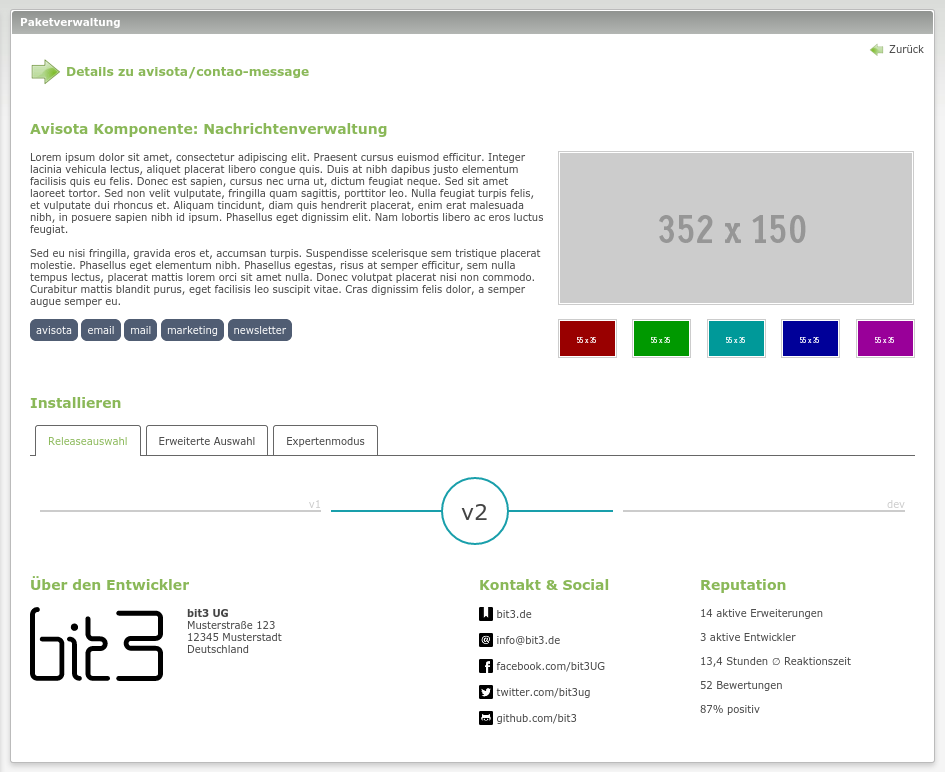
\includegraphics[width=\textwidth]{bilder/mockup-details-1}
  \caption{Mockup: Prototyp für neue Detailansicht mit einfacher Versionsauswahl}
\end{figure}

\begin{figure}[p]
  \centering
  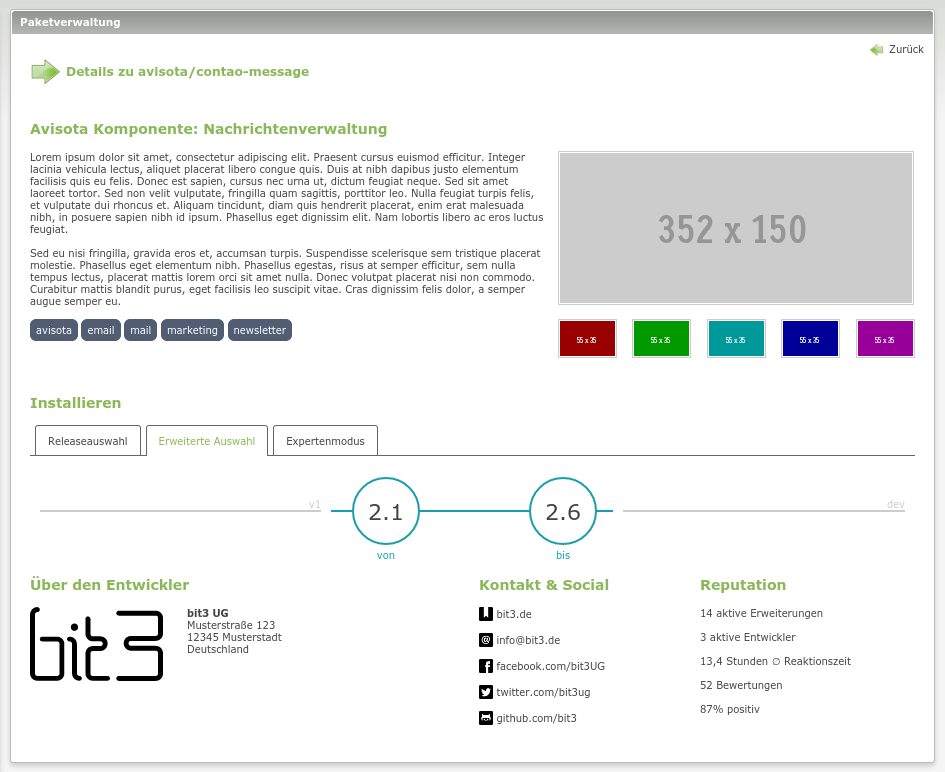
\includegraphics[width=\textwidth]{bilder/mockup-details-2}
  \caption{Mockup: Prototyp für neue Detailansicht mit erweiterter Versionsauswahl}
\end{figure}

\begin{figure}[p]
  \centering
  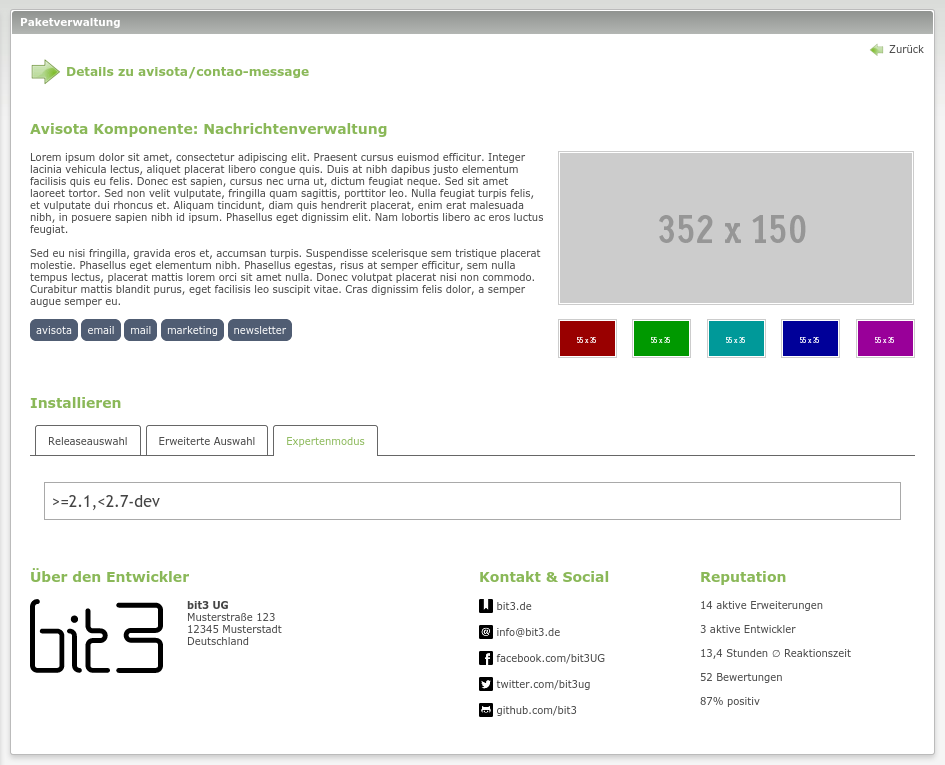
\includegraphics[width=\textwidth]{bilder/mockup-details-3}
  \caption{Mockup: Prototyp für neue Detailansicht mit Versionseingabe für Experten}
\end{figure}

\pagebreak

\subsubsection[Milestone 1.4 - Verbesserte Übersicht installierter Pakete]{Milestone 1.4\footnotemark - Verbesserte Übersicht installierter Pakete}
\footnotetext{\hreflink{https://c-c-a.org/ccc-milestone-1-4}}
\label{subsec:ccc-milestone-1.4}

Die Übersicht der installierten Pakete wurde bereits deutlich verbessert. Sowohl technisch als auch von der Benutzerführung lässt sie doch etwas zu wünschen übrig. Hier soll auch die Benutzerführung und Übersichtlichkeit weiter verbessert und vereinfacht werden.

\subsubsection[Milestone 1.5 - Update Assistent]{Milestone 1.5\footnotemark - Update Assistent}
\footnotetext{\hreflink{https://c-c-a.org/ccc-milestone-1-5}}
\label{subsec:ccc-milestone-1.5}

Updates die bspw. Einstellungen migrieren wurden bisher transparent vom CCP durchgeführt. Dies hat in der Vergangenheit unter anderem zu Problemen geführt. Wir möchten diese in einen Update Assistent auslagern, welcher den Administrator über die notwendigen Updates aufklärt und ihn leitet. Auch die Möglichkeit Updates auszulassen wird es geben, damit schaffen wir die Möglichkeit \textit{optionale Empfehlungen} zu geben.

\subsubsection[Milestone 1.6 - Installationsprozess]{Milestone 1.6\footnotemark - Installationsprozess}
\footnotetext{\hreflink{https://c-c-a.org/ccc-milestone-1-6}}
\label{subsec:ccc-milestone-1.6}

Beim Installationsprozess (also dann wenn composer ausgeführt wird) möchten wir einige Verbesserungen an der Benutzerführung und der Technik durchführen. Dabei steht vor allem die Kompatibilität zu verschiedenen Shared Hostern im Vordergrund.

\subsubsection[Milestone 1.7 - Suche verbessern]{Milestone 1.7\footnotemark - Suche verbessern}
\footnotetext{\hreflink{https://c-c-a.org/ccc-milestone-1-7}}
\label{subsec:ccc-milestone-1.7}

Die Suche ist momentan schwierig - milde ausgedrückt. Die Suche soll mit Hilfe von Ajax und zusätzlichen Filtermöglichkeiten deutlich verbessert werden, so dass es möglich sein wird gezielter zu suchen.

\paragraph{Mockups} ~\\
Nachfolgend möchten wir einen Ausblick auf interne Entwürfe geben, die auf Basis interner Diskussionen und Tickets entstanden sind.

\begin{danger}
Die Mockups sind als Prototypen zu betrachten. \\
Die Entgültige Version kann von den hier gezeigten Screenshots abweichen!
\end{danger}

\begin{figure}[p]
  \centering
  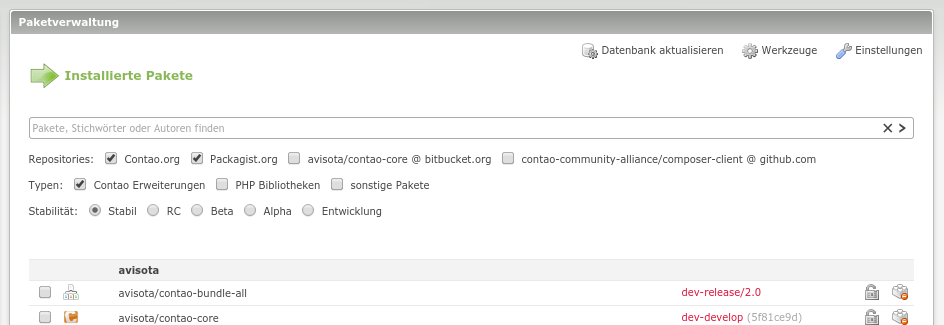
\includegraphics[width=\textwidth]{bilder/mockup-search-bar}
  \caption{Mockup: Prototyp für neue Suchleiste}
\end{figure}

\begin{figure}[p]
  \centering
  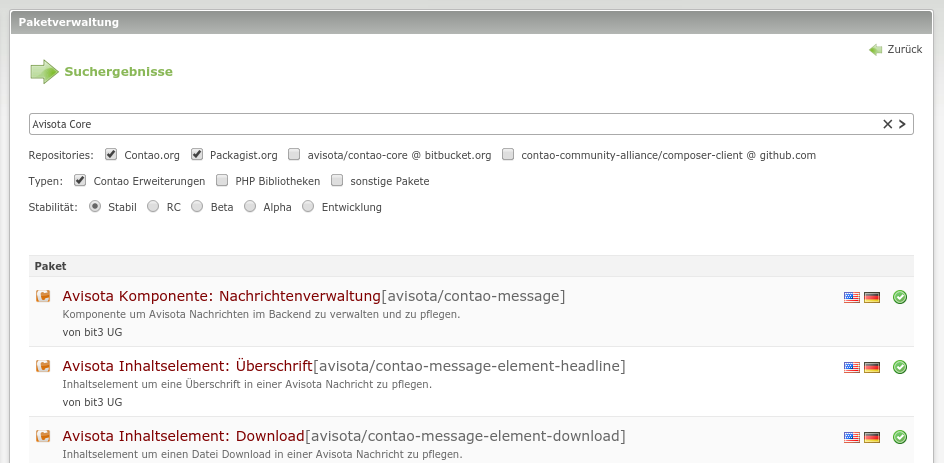
\includegraphics[width=\textwidth]{bilder/mockup-search-result}
  \caption{Mockup: Prototyp für neue Suchergebnis}
\end{figure}

\pagebreak

\subsubsection[Milestone 1.8 - Mehrsprachige Beschreibung]{Milestone 1.8\footnotemark - Mehrsprachige Beschreibung}
\footnotetext{\hreflink{https://c-c-a.org/ccc-milestone-1-8}}
\label{subsec:ccc-milestone-1.8}

Diese Position steht in Zusammenhang mit \nameref{subsec:ccc-milestone-1.3}. Dabei geht es um die Möglichkeit, eine ausführliche Beschreibung innerhalb der Detailansicht anzeigen zu können und das auch noch Mehrsprachig.

\subsubsection[Milestone 1.9 - Upgrade von Paketen]{Milestone 1.9\footnotemark - Upgrade von Paketen}
\footnotetext{\hreflink{https://c-c-a.org/ccc-milestone-1-9}}
\label{subsec:ccc-milestone-1.9}

Momentan wird in der Übersicht der installierten Pakete nicht angezeigt, ob ein Update zur Verfügung steht. Man muss quasi in regelmäßigen Abständen auf \uquot{Pakete aktualisieren} klicken um immer aktuell zu bleiben. Hier soll eine entsprechende Ansicht mit entsprechender Benutzerführung geschaffen werden.

\subsubsection[Milestone 1.10 - Werkzeuge]{Milestone 1.10\footnotemark - Werkzeuge}
\footnotetext{\hreflink{https://c-c-a.org/ccc-milestone-1-10}}
\label{subsec:ccc-milestone-1.10}

Unter \emph{Werkzeuge} verstehen wir verschiedene Aktionen, die im Zusammenhang mit Composer zur Wartung und Fehlerbehebung wichtig sind. Hier sollen einige neue hilfreiche Werkzeuge geschaffen werden.

\subsubsection[Milestone 1.11 - Unterstützung von Drittanbieter-Repositories]{Milestone 1.11\footnotemark - Unterstützung von Drittanbieter-Repositories}
\footnotetext{\hreflink{https://c-c-a.org/ccc-milestone-1-11}}
\label{subsec:ccc-milestone-1.11}

Durch manuelles verändern der composer.json ist es jetzt schon möglich Drittanbieter-Repositories zu nutzen, um bspw. kommerzielle Pakete über Composer zu installieren. Im Rahmen dieser Position sollen die entsprechenden Hilfmittel geschaffen werden, Drittanbieter-Repositories auf einfache Art und Weise hinzuzufügen und zu verwalten.

\subsubsection[Milestone 1.12 - Asset Verwaltung]{Milestone 1.12\footnotemark - Asset Verwaltung}
\footnotetext{\hreflink{https://c-c-a.org/ccc-milestone-1-12}}
\label{subsec:ccc-milestone-1.12}

Installiert man Assets über Composer (bspw. Bootstrap oder Foundation) hat man das Problem, dass man auf die CSS/JS Dateien im vendor Verzeichnis nicht direkt zugreifen kann. Die well-known Dateitypen wurden zwar mittlerweile freigegeben, es kann aber immer noch zu Problemen führen. Wir möchten eine Asset Verwaltung einrichten, mit der es möglich sein wird diese Assets direkt im assets Verzeichnis nutzbar zu machen.

\subsubsection[Milestone 1.13 - NPM/Bower Unterstützung]{Milestone 1.13\footnotemark - NPM/Bower Unterstützung}
\footnotetext{\hreflink{https://c-c-a.org/ccc-milestone-1-13}}
\label{subsec:ccc-milestone-1.13}

Es gibt ein Composer Plugin\footnote{\hreflink{https://github.com/francoispluchino/composer-asset-plugin}} mit dem es möglich ist, gezielt NPM und Bower Pakete mittels Composer zu installieren. Wir möchten dieses Plugin im CCC speziell unterstützen so dass es möglich sein wird ohne großen Aufwand NPM und Bower Pakete zu suchen und zu nutzen.

\pagebreak

\subsection{Entwicklung CCP}
\label{subsec:ccp}

Die Weiterentwicklung des CCP erfolgt in Meilensteinen, die auf github bereits festgehalten wurden. Hier folgt eine kurze Beschreibung der jeweiligen Meilensteine, detaillierte Informationen über deren Inhalt kann dem Ticketsystem auf github entnommen werden.

\subsubsection[Milestone 3.0 alpha - Verschlankung]{Milestone 3.0 alpha\footnotemark - Verschlankung}
\footnotetext{\hreflink{https://c-c-a.org/ccp-milestone-3-0-alpha}}
\label{subsec:ccp-milestone-3.0-alpha}

Aktuell enthällt das Plugin die ganze Migrationslogik. Das führte vor allem in Bezug auf Contao 4 bereits zu Problemen. Deshalb soll die ganze Migrationslogik in den CCC (Milestone 1.5) und das neu entstehende MTK einfließen.

\subsubsection[Milestone 3.0 beta - Refactoring]{Milestone 3.0 beta\footnotemark - Refactoring}
\footnotetext{\hreflink{https://c-c-a.org/ccp-milestone-3-0-beta}}
\label{subsec:ccp-milestone-3.0-beta}

Das aktuelle Vorgehen des Installers, der im Plugin mitgeliefert wird ist aktuell \uquot{nicht optimal}. Unter anderem ist es nicht mehr möglich die Konsolenparameter \texttt{--prefer-dist} und \texttt{--prefer-source} zu verwenden. Deshalb müssen die Installer umgeschrieben werden. In dem Zusammenhang sollen auch ein paar neue Funktionen entstehen, bspw. ein Installationsprotokoll, mit dem man nachvollziehen kann, welche Pakete wann und wie installiert, aktualisiert und deinstalliert wurden.

\pagebreak

\subsection{Entwicklung CCR}
\label{subsec:ccr}

\subsubsection{Milestone 1 - Installation, Einrichtung, Branding}
\label{subsec:ccr-milestone-1}

Auf dem von der Contao Association betriebenen Community Server soll ein Packagist Server installiert und eingerichtet werden. Dieser soll außerdem für das Contao Projekt gebrandet werden.

\begin{description}
\item[Ticket] contao-community-alliance/composer-reposititory\#1\footnote{\hreflink{https://c-c-a.org/ccr-issue-1}}
\end{description}

\subsubsection{Milestone 2 - Theming und Suche}
\label{subsec:ccr-milestone-2}

Bei Packagist gibt es einen vielversprechenden, leider eingefrorenes Redesign\footnote{\hreflink{https://github.com/composer/packagist/pull/331}}. Das möchten wir aufgreifen und fortführen. Gleichzeitig wollen wir die Suche in Packagist verbessern und mehr Filtermöglichkeiten einbauen. Diese sollen dann im CCC \nameref{subsec:ccc-milestone-1.7} genutzt werden, um die Suche im Backend zu verbessern.

\subsubsection{Milestone 3 - Detaillierte Projektbeschreibung}
\label{subsec:ccr-milestone-3}

Aktuell kann man nur eine \uquot{kurze} Beschreibung in einer Sprache festlegen. Basierent auf einem Vorstoß\footnote{\hreflink{https://github.com/composer/composer/issues/1954}} den wir bereits einmal in diese Richtung gemacht hatten, möchten wir die Möglichkeit bieten detaillierte, mehrsprachige Projektbeschreibungen zu definieren.

\vspace{1cm}

\begin{info}
Die weiteren Punkte sind noch nicht im Detail geplant, es gibt bisher nur einige Ideen wo die Reise hin gehen soll. Siehe Abschnitt \nameref{sec:long-term-goals}.
\end{info}

\pagebreak

\subsection{Entwicklung CJG}
\label{subsec:cjg}

\subsubsection{Milestone 1 - Umsetzung}
\label{subsec:cjg-milestone-1}

Der composer.json Generator ist ein Web-Tool, in das ein Entwickler seine Repository URL einträgt und dann eine auf sein Repository zugeschnittene composer.json erhält. Der Generator analysiert das Repository und nimmt die entsprechenden Eintragungen vor. Zusätzlich soll dem Entwickler durch eine inline-Dokumentation die composer.json näher gebracht werden.

\begin{description}
\item[Ticket] contao-community-alliance/composer.json-generator\#1\footnote{\hreflink{https://c-c-a.org/cjg-issue-1}}
\end{description}

\subsection{Entwicklung DUT}
\label{subsec:dut}

\begin{emquotation}
Warum brauchen wir ein eigenständiges Tool für das Datenbankupdate? \\
\hspace*{\fill}Das haben wir doch schon?
\end{emquotation}

Ja das ist richtig, wir wollen das Rad ja auch nicht neu erfinden. Genau genommen wollen wir den DCA Extractor aus Contao 4 extrahieren, aufarbeiten und mit dem Doctrine Schema Tool \uquot{verheiraten}.\\
Oder mit anderen Worten: Wir wollen hier auf die existierende Funktion von Contao aufbauen und verbessern. Das wichtigste Dabei ist allerdings, dass wir mit diesem Tool vom Contao Framework selbst unabhängig werden wollen. Das ist vor allem für den \textit{Standalone Modus} wichtig, der auch ohne funktionierendes Contao System lauffähig sein soll. Aber auch für Contao 4 gibt das uns Entwicklern mehr Möglichkeiten.

\subsubsection{Milestone 1 - Umsetzung}
\label{subsec:dut-milestone-1}

\begin{description}
\item[Ticket] contao-community-alliance/database-update-tool\#1\footnote{\hreflink{https://c-c-a.org/dut-issue-1}}
\end{description}

\pagebreak

\subsection{Entwicklung MTK}
\label{subsec:mtk}

\begin{emquotation}
Warum brauchen wir ein Migration Toolkit? Reicht die runonce.php nicht aus?
\end{emquotation}

Die \texttt{runonce.php} ist nicht immer einfach zu handhaben. Im Fehlerfall kann es passieren, dass wichtige Updates gar nicht ausgeführt werden ohne das der Administrator etwas davon mit bekommt, außer dass eine Extension ggf. nicht mehr richtig funktioniert. Im schlimmsten Fall kann es sogar dazu führen, dass das Install-Tool / Datenbankupdate nicht mehr aufrufbar ist (=weiße Seite) und erst nach löschen von defekten \texttt{runonce.php} Dateien wieder funktioniert.\\
Das Migration Toolkit verfolgt drei Ziele:

\begin{dinglist}{'64}
\item Dem Administrator wieder mehr Kontrolle über die Migrationsschritte nach einem Update einräumen.
\item Dem Administrator ausreichende Informationen bei fehlerhafte Updates bereitstellen.
\item Dem Entwickler das Bereitstellen von Migrationsschritten zu vereinfachen.
\end{dinglist}

Nicht selten kam es in der Vergangenheit immer wieder vor, dass \texttt{runonce.php's} nicht korrekt ausgeführt wurden. Oft zeigt sich dies in einem Fehlverhalten von Erweiterungen oder sogar dem Fehlen von (alten) Daten. In vielen Fällen konnten derartige Probleme mit dem erneuten Installieren von Erweiterungen behoben werden, aber auch nicht immer. Manchmal muss der Administrator auch selbst Hand anlegen.\\
Dadurch dass wir die einzelnen Migrationsschritte atomarisieren wollen (d.h. jeder Schritt wird einzeln ausgeführt) können wir dem Administrator detaillierte Informationen bereitstellen wenn etwas schief gelaufen ist. Das hilft dem Administrator bei der Behebung von Fehlern, aber auch dem Entwickler der die Fehler in einem Update beheben kann.

\subsubsection{Milestone 1 - Umsetzung}
\label{subsec:mtk-milestone-1}

\begin{description}
\item[Ticket] contao-community-alliance/migration-toolkit\#1\footnote{\hreflink{https://c-c-a.org/mtk-issue-1}}
\end{description}

\newpage

% --------------------------------------------------------------------------------
%
%     Angebot / Entwicklungspakete
%
% --------------------------------------------------------------------------------

\section{Angebot / Entwicklungspakete}
\label{sec:offer}

\subsection{Sprint 1: Reworking and Refactoring}
\label{subsec:sprint-1}

Im ersten Sprint soll die Oberfläche des CCC überarbeitet werden und die Implementierung des CCP überarbeitet werden.
Außerdem soll die Dokumentation zusammen geführt und die zugehörigen Teilabschnitten ausgearbeitet werden.

\begin{tabular*}{\textwidth}{@{\extracolsep{\fill} }p{.8\textwidth}r}
\textbf{Position} & \textbf{Preis} \\
\hline

\textbf{CCC} \newline
\tabitem \nameref{subsec:ccc-milestone-1.0-beta} \newline
\tabitem \nameref{subsec:ccc-milestone-1.0} \newline
\tabitem \nameref{subsec:ccc-milestone-1.1} \newline
\tabitem \nameref{subsec:ccc-milestone-1.2} \newline
\tabitem \nameref{subsec:ccc-milestone-1.3} \newline
\tabitem \nameref{subsec:ccc-milestone-1.4} \newline
& 6.000 \euro \\
\hline

\textbf{CCP} \newline
\tabitem \nameref{subsec:ccp-milestone-3.0-alpha} \newline
\tabitem \nameref{subsec:ccp-milestone-3.0-beta}
& 3.000 \euro \\
\hline

& \textbf{9.000 \euro}
\end{tabular*}

\subsection{Sprint 2: Contao Repository Server}
\label{subsec:sprint-2}

Im zweiten Sprint soll der CCR installiert, eingerichtet und auf Contao gebrandet werden.

\begin{tabular*}{\textwidth}{@{\extracolsep{\fill} }p{.8\textwidth}r}
\textbf{Position} & \textbf{Preis} \\
\hline

\textbf{CCR} \newline
\tabitem \nameref{subsec:ccr-milestone-1}
& 1.000 \euro \\
\hline

& \textbf{1.000 \euro}
\end{tabular*}

\subsection{Sprint 3: Composer.json Generator}
\label{subsec:sprint-3}

Im dritten Sprint soll der CJG umgesetzt werden und in die Dokumentation eingearbeitet / mit der Dokumentation verknüpft werden.

\begin{tabular*}{\textwidth}{@{\extracolsep{\fill} }p{.8\textwidth}r}
\textbf{Position} & \textbf{Preis} \\
\hline

\textbf{CJG} \newline
\tabitem \nameref{subsec:cjg-milestone-1}
& \sout{3.000 \euro} \\
\hline

& \sout{\textbf{3.000 \euro}}
\end{tabular*}

\begin{success}
\center Der Sprint 3 wird im Falle der Bewilligung von Sprint 1+2 vollständig von der WESTWERK GmbH \& Co. KG finanziert und umgesetzt.
\end{success}

\pagebreak

\begin{info}
Die folgenden Sprints geben eine Aussicht auf das, was im kommenden Jahr noch geplant ist bzw. zur Förderung eingereicht wird.
Im Gegensatz zu \nameref{subsec:sprint-1} und \nameref{subsec:sprint-2} - die beide Voraussetzung für die weitere Entwicklung sind - können die folgenden Sprints in beliebiger Reihenfolge umgesetzt werden.
\end{info}

\begin{danger}
Diese Sprints sollten erst mal nur als grobe Roadmap betrachtet werden. Die Sprints müssen ggf. noch detaillierter ausgearbeitet werden, bevor diese zur Förderung eingereicht werden.
\end{danger}

\subsection{Sprint 4: Upgrade Fähigkeit verbessern}
\label{subsec:sprint-4}

Im vierten Sprint soll die \uquot{Upgrade Fähigkeit} verbessert werden. Das betrifft vor allem die Implementierung des DUT und MTK und deren Integration in den CCC.

\begin{tabular*}{\textwidth}{@{\extracolsep{\fill} }p{.8\textwidth}r}
\textbf{Position} & \textbf{Preis} \\
\hline

\textbf{CCC} \newline
\tabitem \nameref{subsec:ccc-milestone-1.5}
& - \euro \\
\hline

\textbf{DUT} \newline
\tabitem \nameref{subsec:dut-milestone-1}
& - \euro \\
\hline

\textbf{MTK} \newline
\tabitem \nameref{subsec:mtk-milestone-1}
& - \euro \\
\hline

& \textbf{- \euro}
\end{tabular*}

\subsection{Sprint 5: Installationsprozess optimieren}
\label{subsec:sprint-5}

Im fünften Sprint soll der Installationsprozess überarbeitet werden. Hiermit soll vor allem die Kompatibilität und Stabilität des Updateprozesses erhöht werden.

\begin{tabular*}{\textwidth}{@{\extracolsep{\fill} }p{.8\textwidth}r}
\textbf{Position} & \textbf{Preis} \\
\hline

\textbf{CCC} \newline
\tabitem \nameref{subsec:ccc-milestone-1.6}
& - \euro \\
\hline

& \textbf{- \euro}
\end{tabular*}

\subsection{Sprint 6: Suche optimieren}
\label{subsec:sprint-6}

Im sechsten Sprint soll der Suche überarbeitet und deutlich verbessert werden. Hierzu muss sowohl der CCC als auch das CCR angepackt werden.

\begin{tabular*}{\textwidth}{@{\extracolsep{\fill} }p{.8\textwidth}r}
\textbf{Position} & \textbf{Preis} \\
\hline

\textbf{CCC} \newline
\tabitem \nameref{subsec:ccc-milestone-1.7}
& - \euro \\
\hline

\textbf{CCR} \newline
\tabitem \nameref{subsec:ccr-milestone-2}
& - \euro \\
\hline

& \textbf{- \euro}
\end{tabular*}

\subsection{Sprint 7: Detaillierte Projektbeschreibung}
\label{subsec:sprint-7}

Im siebten Sprint soll es ermöglicht werden, detailliertere Projektbeschreibungen zu definieren.

\begin{warning}
Wir empfehlen diesen Sprint nur zusammen mit \nameref{subsec:sprint-6} anzunehmen.
\end{warning}

\begin{tabular*}{\textwidth}{@{\extracolsep{\fill} }p{.8\textwidth}r}
\textbf{Position} & \textbf{Preis} \\
\hline

\textbf{CCC} \newline
\tabitem \nameref{subsec:ccc-milestone-1.8}
& - \euro \\
\hline

\textbf{CCR} \newline
\tabitem \nameref{subsec:ccr-milestone-3}
& - \euro \\
\hline

& \textbf{- \euro}
\end{tabular*}

\subsection{Sprint 8: Anzeige von Updates}
\label{subsec:sprint-8}

Im achten Sprint soll der Anzeige der Installierten Paketen eine Anzeige hinzugefügt werden, welche Pakete aktualisiert werden können (\uquot{Update} innerhalb der gewählten Version) oder auf eine neuere Hauptversion aktualisiert werden können (\uquot{Upgrade} auf die nächste Hauptversion).

\begin{tabular*}{\textwidth}{@{\extracolsep{\fill} }p{.8\textwidth}r}
\textbf{Position} & \textbf{Preis} \\
\hline

\textbf{CCC} \newline
\tabitem \nameref{subsec:ccc-milestone-1.9}
& - \euro \\
\hline

& \textbf{- \euro}
\end{tabular*}

\subsection{Sprint 9: Mehr Werkzeuge}
\label{subsec:sprint-9}

Im neunten Sprint sollen weitere hilfreiche \emph{Werkzeuge} zum CCC hinzugefügt werden.

\begin{tabular*}{\textwidth}{@{\extracolsep{\fill} }p{.8\textwidth}r}
\textbf{Position} & \textbf{Preis} \\
\hline

\textbf{CCC} \newline
\tabitem \nameref{subsec:ccc-milestone-1.10}
& - \euro \\
\hline

& \textbf{- \euro}
\end{tabular*}

\subsection{Sprint 10: Drittanbieter-Repositories}
\label{subsec:sprint-10}

Im zehnten Sprint sollen Drittanbieter-Repositories (bspw. von kommerziellen Anbieter) besser vom CCC unterstützt werden.

\begin{tabular*}{\textwidth}{@{\extracolsep{\fill} }p{.8\textwidth}r}
\textbf{Position} & \textbf{Preis} \\
\hline

\textbf{CCC} \newline
\tabitem \nameref{subsec:ccc-milestone-1.11}
& - \euro \\
\hline

& \textbf{- \euro}
\end{tabular*}

\subsection{Sprint 11: Asset Verwaltung}
\label{subsec:sprint-11}

\begin{warning}
In Contao 4 gibt es bereits ein Deployment von öffentlichen Assets. Abhängig von der Entwicklung von Contao 4 kann sich dieser Sprint noch verändern oder sogar gänzlich weg fallen, wenn es für Contao 3 nicht mehr relevant sein sollte.
\end{warning}

Aktuell ist der Zugriff auf Assets innerhalb des \texttt{TL\_ROOT/composer/vendor} Verzeichnisses zwar möglich, weil wir die \textit{well-known} Dateitypen freigegeben haben. Im elften Sprint wollen wir es ermöglichen, Assets automatisiert vom CCC oder CCP in das öffentliche \texttt{TL\_ROOT/assets} Verzeichnis kopieren zu lassen, wenn ein Drittanbieter-Paket mit Assets installiert wird.

\begin{tabular*}{\textwidth}{@{\extracolsep{\fill} }p{.8\textwidth}r}
\textbf{Position} & \textbf{Preis} \\
\hline

\textbf{CCC} \newline
\tabitem \nameref{subsec:ccc-milestone-1.12}
& - \euro \\
\hline

& \textbf{- \euro}
\end{tabular*}

\subsection{Sprint 12: NPM/Bower Support}
\label{subsec:sprint-12}

Im zwölften Sprint wollen wir NPM und Bower Support in den CCC einbauen.

\begin{tabular*}{\textwidth}{@{\extracolsep{\fill} }p{.8\textwidth}r}
\textbf{Position} & \textbf{Preis} \\
\hline

\textbf{CCC} \newline
\tabitem \nameref{subsec:ccc-milestone-1.13}
& - \euro \\
\hline

& \textbf{- \euro}
\end{tabular*}

\newpage

% --------------------------------------------------------------------------------
%
%     Glossar
%
% --------------------------------------------------------------------------------

\section{Glossar}

\begin{description}
\item[CCA] Contao Community Alliance \\
\hreflink{https://c-c-a.org}
\item[CCC] Contao Composer Client \\
\hreflink{https://github.com/contao-community-alliance/composer-client}
\item[CCP] Contao Composer Plugin \\
\hreflink{https://github.com/contao-community-alliance/composer-plugin}
\item[CCR] Contao Composer Repository \\
\hreflink{https://github.com/contao-community-alliance/composer-reposititory}
\item[CCD] Contao Composer Dokumentation \\
\hreflink{https://github.com/contao-community-alliance/composer-docs-de}
\item[CJG] Composer.json Generator \\
\hreflink{https://github.com/contao-community-alliance/composer.json-generator}
\end{description}

\end{document}
